\section{Introduction}
\label{cha:intro}

While convex losses for binary classification have dominated the
machine learning literature for well over a decade, it is well-known
that convex losses are sensitive to outliers.  Popular convex
solutions for binary classification problems (with noise) include
soft-margin SVMs~\cite{} and logistic regression~\cite{}.
Unfortunately, convex losses are known to be prone to
outliers~\cite{wu07,servidio?} as demonstrated empirically in
Figure~\ref{fig:svm_failure}.  Here, both the SVM and logistic
regression find a solution that is highly suboptimal.
% BPM: find a single weight vector that has properties similar to
%      Bayes optimal classifier for 

Why does this happen?  Figure~\ref{}.

%%%%%%%%%%%%%%%%%%%%%%%%%%%%%%%%%%%%%%%%%%%%%%%%%%%%%%%%%%%%%%%%%%%%
\begin{figure}[t!]
\vspace{-3mm}
\hspace{-3mm} 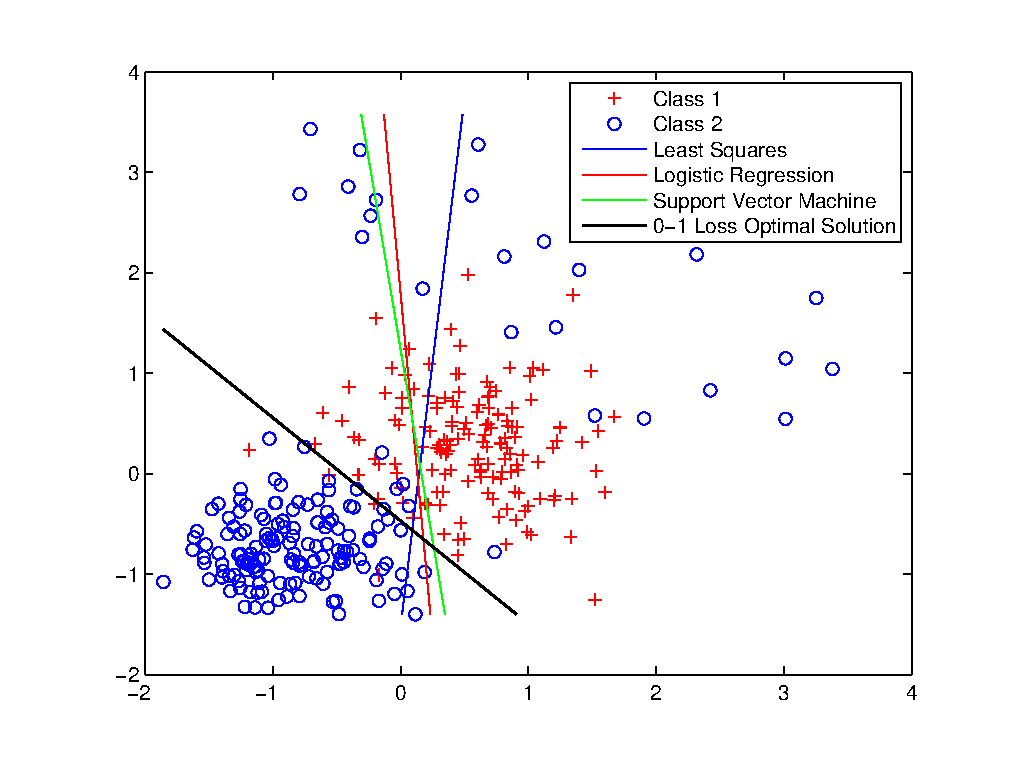
\includegraphics[width=0.50\textwidth]{images/fig11_svm_failure2.eps}
\vspace{-9mm}
\caption{ \footnotesize Training data consisting of 300 points of two
  classes, 10\% of which are outliers.  All convex losses (least
  squares, logistic regression, SVM) are skewed by the outliers and
  their decision boundaries make $\geq$ 61 classification errors,
  whereas the optimal 0--1 loss solution makes 39 errors with a decision
  boundary that is robust to the outliers.}
\label{fig:svm_failure}
\vspace{-3mm}
\end{figure}
%%%%%%%%%%%%%%%%%%%%%%%%%%%%%%%%%%%%%%%%%%%%%%%%%%%%%%%%%%%%%%%%%%%%

Do we have to worry about outliers?  Examples include testing whether
a patient has cancer, or testing whether a locomotive wheel has
crack. Outliers in these cases may come from abnormal noise or defect
of equipments, from human mistakes, etc. These examples show that
classifiers which are robust to outliers are needed.

0--1 loss to the rescue in Figure~\ref{fig:svm_failure}.  Why not
optimize 0--1 loss?  Figure~\ref{fig:complex_shape}.  In fact, it is
NP--hard to optimize 0--1 loss directly \cite{Feldman,nphard}, and
most of the current algorithms solve this problem by minimizing a
convex surrogate of the 0--1 loss function, because convexity makes
them computationally efficient \cite{Bartlett}.

%%%%%%%%%%%%%%%%%%%%%%%%%%%%%%%%%%%%%%%%%%%%%%%%%%%%%%%%%%%%%%%%%%%%
\begin{figure}[t!]
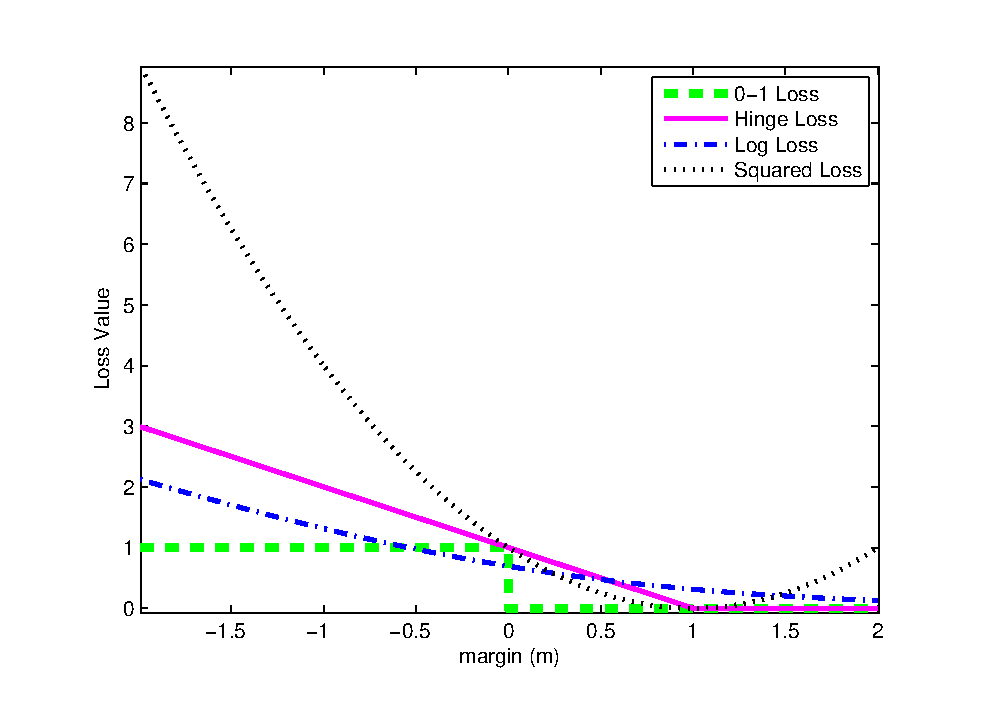
\includegraphics[width=0.50\textwidth]{images/fig13_losses.eps}
\caption{ \footnotesize Different loss functions: hinge loss (SVM),
  log loss (logistic regression), squared loss (linear regression),
  and 0--1 loss.  }
\label{fig:losses}
\end{figure}
%%%%%%%%%%%%%%%%%%%%%%%%%%%%%%%%%%%%%%%%%%%%%%%%%%%%%%%%%%%%%%%%%%%%

Nonetheless, there exist numerous practical methods for attacking
such problems.  In particular, we contribute:

Branch and bound: good initialization plus heuristics: best-first and
loss propagation.  Optimal solutions up to a few hundred data points.

Reformulation of the problem to enable combinatorial search that
searches through all legal combinations of separating hyperplanes,
with ordering, yields efficient solutions for low dimensional
problems.  Also propose a two-layer approximation having polynomial
worst-case running time allowing it to scale to ten thousand data
points with a good approximation to the optimal solution.

Development of a smooth, differentiable loss relaxation of 0--1 loss
that can approximate it to an arbitrarily level of precision and a
coordinate descent approach with techniques for escaping local
optima. Similar approximation quality as that of the combinatorial
search approximation, while significantly faster: quadratic in
worst-case but much faster on average.  Can solve problems of up to
about a hundred thousand data points.

Empirically, we compare our proposed algorithms to logistic
regression, SVM, and the Bayes point machine showing that the proposed
0--1 loss optimization algorithms perform at least comparably and
offer a clear advantage in the presence of outliers.  To this end, we
believe this work reiterates the potential importance of non-convex
losses and their properties while partially challenging long-held
notions that non-convex losses are difficult to optimize.

%%%%%%%%%%%%%%%%%%%%%%%%%%%%%%%%%%%%%%%%%%%%%%%%%%%%%%%%%%%%%%%%%%%%
\begin{figure}[t!]
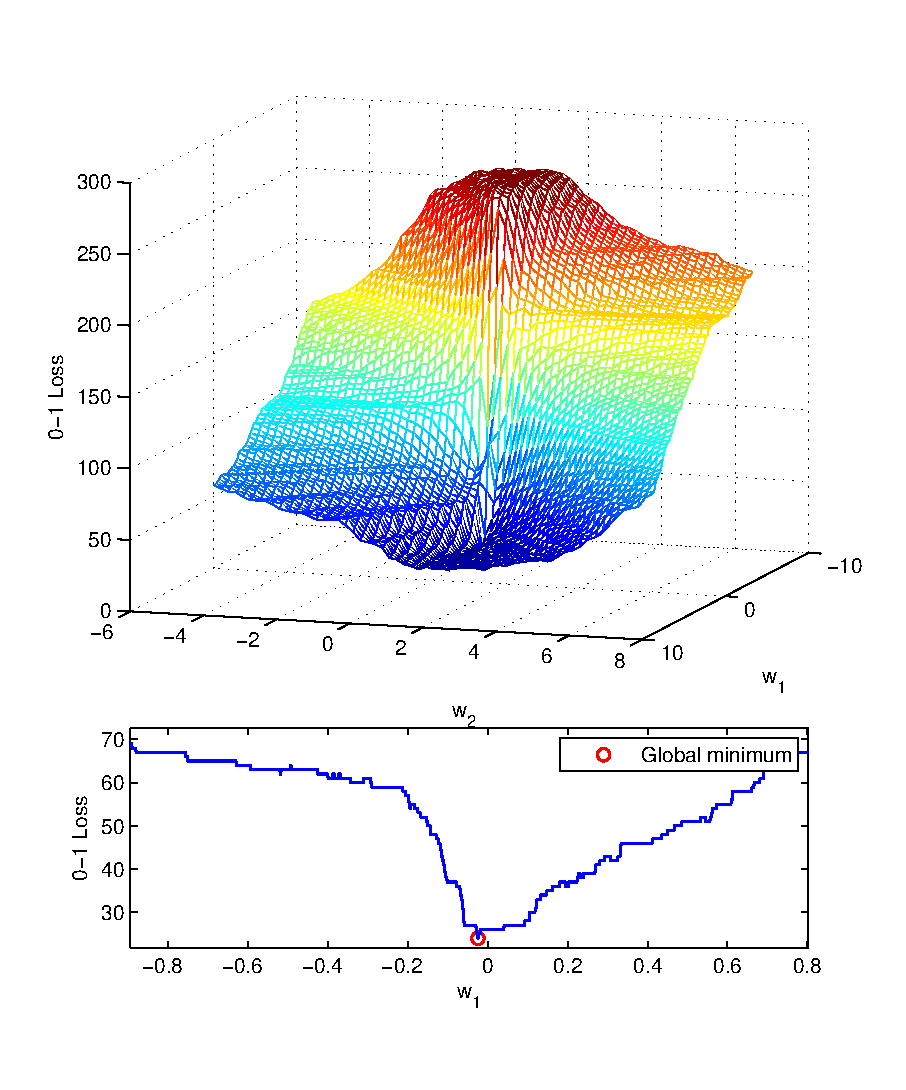
\includegraphics[width=0.50\textwidth]{images/fig14_complexshape.eps}
\caption{ \footnotesize The complex shape of 0--1 loss function.  The
  top figure plots 0--1 loss function of a two-dimensional dataset as
  a function of two varying weights $w_1$ and $w_2$ (that control the
  decision boundary). The bottom figure plots the same function in
  more detailed scale with $w_2$ held fixed at optimal value. As can
  be seen, the 0--1 loss function has a complex shape with numerous
  local optima, higher dimensionalities would lead to even more
  complex surfaces.  }
\label{fig:complex_shape}
\end{figure}
%%%%%%%%%%%%%%%%%%%%%%%%%%%%%%%%%%%%%%%%%%%%%%%%%%%%%%%%%%%%%%%%%%%%

